\documentclass[12pt,a4paper]{article}

% --- Encodage et langue ---
\usepackage[utf8]{inputenc}
\usepackage[T1]{fontenc}
\usepackage{lmodern}

% --- Maths ---
\usepackage{amsmath,amssymb,amsthm}

% --- Mise en page ---
\usepackage[top=2.5cm,bottom=2.5cm,left=2.8cm,right=2.8cm]{geometry}
\usepackage{parskip}

% --- Tableaux ---
\usepackage{booktabs}
\usepackage{array}
\usepackage{multirow}

% --- Figures et couleurs ---
\usepackage{tikz}
\usetikzlibrary{arrows.meta, positioning, decorations.pathreplacing, calc, fit, backgrounds}
\usepackage{xcolor}
\usepackage{pgfplots}
\pgfplotsset{compat=1.18}

% --- Liens ---
\usepackage{hyperref}
\hypersetup{colorlinks=true, linkcolor=blue!60!black, citecolor=blue!60!black}

% --- Environnements théorème ---
\newtheorem{theorem}{Théorème}[section]
\newtheorem{lemma}[theorem]{Lemme}
\newtheorem{corollary}[theorem]{Corollaire}
\theoremstyle{remark}
\newtheorem{remark}{Remarque}[section]
\newtheorem{example}{Exemple}[section]

% --- Macros ---
\newcommand{\Inc}{\ensuremath{\mathrm{Include}}}
\newcommand{\Exc}{\ensuremath{\mathrm{Exclude}}}
\newcommand{\vbar}{\bar{v}}
\newcommand{\ps}{\text{ p.s.}}

% ======================================================
\begin{document}
% ======================================================

\begin{center}
  {\LARGE\bfseries Démonstration de convergence}\\[6pt]
  {\large de la règle d'apprentissage à 4 cas}\\[4pt]
  {\large\itshape Opérateurs IDENTITY et NOT --- Cas sans bruit et avec bruit}\\[12pt]
  {\normalsize Analyse par chaînes de Markov}
\end{center}

\vspace{1em}
\hrule
\vspace{1.5em}

\tableofcontents

\newpage

% ======================================================
\section{Mise en place}
% ======================================================

\subsection{Variables et automates}

On considère une seule caractéristique binaire $x \in \{0,1\}$, associée à un label cible
$y \in \{0,1\}$, dans le \textbf{cas sans bruit} : le label est déterministe, c'est-à-dire $y = f(x)$
pour une fonction booléenne fixée $f$.  On note
\[
  P(x = 1) = c, \quad c \in (0,1).
\]

La clause est gouvernée par deux \textbf{automates de Tsetlin} :
\begin{itemize}
  \item $v$\,: associé au littéral $x$, d'état $s_1 \in \{1,\ldots,2N\}$,
  \item $\vbar$\,: associé au littéral $\neg x$, d'état $s_2 \in \{1,\ldots,2N\}$.
\end{itemize}
La règle de décision est :
\[
  \mathrm{included}(s) =
  \begin{cases} 1 & \text{si } s > N \quad [\text{action } \Inc], \\ 0 & \text{si } s \le N \quad [\text{action } \Exc]. \end{cases}
\]

\subsection{Sémantique de la clause}

La sortie de la clause est :
\[
  C(x) = \begin{cases}
    x     & \text{si } v = \Inc,\;\vbar = \Exc \quad \longrightarrow \text{[IDENTITY]} \\
    \neg x & \text{si } v = \Exc,\;\vbar = \Inc \quad \longrightarrow \text{[NOT]}       \\
    1     & \text{si } v = \Exc,\;\vbar = \Exc \quad \longrightarrow \text{[tautologie]} \\
    0     & \text{si } v = \Inc,\;\vbar = \Inc \quad \longrightarrow \text{[contradiction]}
  \end{cases}
\]

\begin{figure}[h]
\centering
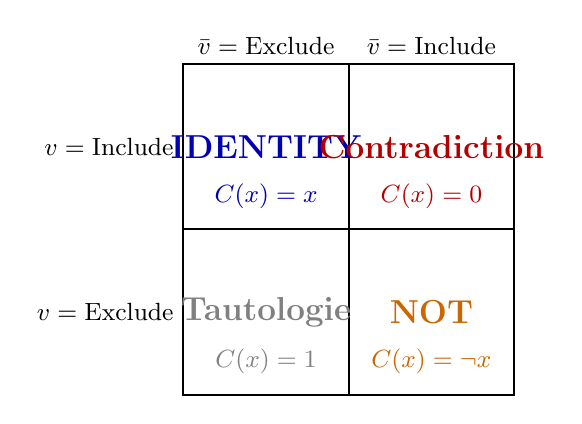
\begin{tikzpicture}[scale=1.05]
  % Grid
  \draw[thick] (0,0) rectangle (4,4);
  \draw[thick] (2,0) -- (2,4);
  \draw[thick] (0,2) -- (4,2);
  % Labels axes
  \node[above] at (1,4) {\small $\vbar = \Exc$};
  \node[above] at (3,4) {\small $\vbar = \Inc$};
  \node[left]  at (0,3) {\small $v = \Inc$};
  \node[left]  at (0,1) {\small $v = \Exc$};
  % Contents
  \node[font=\bfseries\large, text=blue!70!black] at (1,3) {IDENTITY};
  \node[font=\small, text=blue!70!black] at (1,2.4) {$C(x)=x$};
  \node[font=\bfseries\large, text=red!70!black]  at (3,3) {Contradiction};
  \node[font=\small, text=red!70!black]  at (3,2.4)  {$C(x)=0$};
  \node[font=\bfseries\large, text=gray]       at (1,1) {Tautologie};
  \node[font=\small, text=gray]       at (1,0.4)  {$C(x)=1$};
  \node[font=\bfseries\large, text=orange!80!black] at (3,1) {NOT};
  \node[font=\small, text=orange!80!black] at (3,0.4)  {$C(x)=\neg x$};
\end{tikzpicture}
\caption{Quatre configurations possibles de $(v, \vbar)$ et leur sémantique logique.}
\label{fig:config}
\end{figure}

% ======================================================
\section{La règle d'apprentissage à 4 cas}
% ======================================================

À chaque exemple $(x,y)$ observé, les automates $v$ et $\vbar$ sont mis à jour
\emph{simultanément} selon le tableau suivant (implémenté dans \texttt{Clause::update}).

\begin{center}
\begin{tabular}{ccll}
\toprule
$x$ & $y$ & Action sur $v$ & Action sur $\vbar$ \\
\midrule
0 & 0 & \texttt{versInclude}$(S)$ & \texttt{versExclude}$(S)$ \\
0 & 1 & \texttt{versExclude}$(\alpha)$ & rien \\
1 & 0 & \texttt{versExclude}$(S)$ & \texttt{versInclude}$(S)$ \\
1 & 1 & rien & \texttt{versExclude}$(\alpha)$ \\
\bottomrule
\end{tabular}
\end{center}

où $S, \alpha \in (0,1]$ sont deux paramètres fixes. L'opérateur \texttt{versInclude}$(p)$
déplace l'état d'une unité vers la droite avec probabilité $p$ (borné par $2N$);
\texttt{versExclude}$(p)$ le déplace vers la gauche avec probabilité $p$ (borné par $1$).

\begin{lemma}[Découplage vis-à-vis de la sortie de la clause]\label{lem:decoupling}
L'action appliquée à $v$ (resp. $\vbar$) à l'instant $t$ ne dépend que du couple
$(x_t, y_t)$. Elle ne dépend \emph{ni} de la valeur $C(x_t)$ de la clause, \emph{ni}
de l'état courant de l'autre automate.
\end{lemma}

\begin{proof}
Vérification directe : chaque ligne du tableau est indexée uniquement par $(x,y)$,
sans aucune référence à $C(x)$ ou à l'état de l'automate complémentaire.
\end{proof}

\begin{remark}\label{rem:difference_tm}
Cette propriété constitue la \textbf{différence structurelle majeure} avec la règle
originale de la Tsetlin Machine \cite{granmo2018,zhang2021}, où le retour de Type~II
dépend explicitement de $C(x)$, donc de l'état combiné des deux automates.  Cette
dépendance oblige, dans l'analyse de Zhang et al., à distinguer quatre configurations
initiales $(E,E),(E,I),(I,E),(I,I)$ et à construire une chaîne de Markov conditionnelle
pour chacune (Figure~5 dans \cite{zhang2021}).  Le Lemme~\ref{lem:decoupling} montre
qu'une seule chaîne par automate suffit ici, valable uniformément pour toute configuration
initiale.
\end{remark}

% ======================================================
\section{Lemme de convergence fondamental}
% ======================================================

\begin{lemma}[Chaîne à direction unique]\label{lem:convergence}
Soit une chaîne de Markov homogène sur $\{1,\ldots,2N\}$, à probabilités de transition
intérieures constantes :
\begin{itemize}
  \item vers la droite : $p^+ \ge 0$,
  \item vers la gauche : $p^- \ge 0$,
  \item sur place : $1 - p^+ - p^-$.
\end{itemize}
\begin{enumerate}
  \item[\textup{(a)}] Si $p^- = 0$ et $p^+ > 0$, la chaîne atteint l'état $2N$ en temps fini p.s.\ et y reste indéfiniment.
  \item[\textup{(b)}] Si $p^+ = 0$ et $p^- > 0$, la chaîne atteint l'état $1$ en temps fini p.s.\ et y reste indéfiniment.
\end{enumerate}
\end{lemma}

\begin{proof}
Nous traitons le cas~(a) : $p^- = 0$, $p^+ > 0$.
Le cas~(b) se ramène au cas~(a) par réflexion de l'espace d'états (substitution $s \mapsto 2N+1-s$).

\medskip
\textbf{Étape 1 : monotonie de la chaîne.}
Puisque $p^- = 0$, la chaîne ne peut jamais reculer. Formellement, pour tout $t \ge 0$,
\[
  P(s_{t+1} < s_t) = p^- = 0,
\]
donc la suite $(s_t)_{t \ge 0}$ est \emph{presque sûrement non-décroissante}.

\medskip
\textbf{Étape 2 : probabilité d'absorption égale à 1 (fonction harmonique).}

Soit $u_k = P(T < \infty \mid s_0 = k)$ la probabilité d'atteindre $2N$ en temps fini
depuis l'état $k$, où $T = \inf\{t \ge 0 : s_t = 2N\}$.
La condition aux bords est $u_{2N} = 1$.
Pour tout état intérieur $k \in \{1,\ldots,2N-1\}$, la propriété de Markov donne
l'équation harmonique :
\[
  u_k = p^+ \cdot u_{k+1} + (1-p^+) \cdot u_k.
\]
En réarrangeant :
\[
  p^+ \cdot u_k = p^+ \cdot u_{k+1} \quad \Longrightarrow \quad u_k = u_{k+1}
  \qquad \text{pour tout } k < 2N.
\]
On obtient donc la suite constante $u_1 = u_2 = \cdots = u_{2N} = 1$, c'est-à-dire
\[
  \boxed{P(T < \infty \mid s_0 = k) = 1 \qquad \text{pour tout } k \in \{1,\ldots,2N\}.}
\]

\medskip
\textbf{Étape 3 : espérance finie du temps d'atteinte (loi négative binomiale).}

Posons $r = 2N - s_0 \ge 1$ le nombre de pas ascendants nécessaires.
Définissons les temps d'inter-palier successifs : pour $j = 1, \ldots, r$,
\[
  W_j = \min\bigl\{t \ge 1 : s_{\tau_{j-1}+t} = s_0 + j\bigr\},
\]
où $\tau_0 = 0$ et $\tau_j = \tau_{j-1} + W_j$.
Par la propriété de Markov et l'homogénéité des transitions, les $W_j$ sont
\emph{indépendants et identiquement distribués} selon une loi géométrique :
\[
  P(W_j = k) = (1-p^+)^{k-1}\, p^+ \qquad (k \ge 1),
  \qquad
  E[W_j] = \frac{1}{p^+}.
\]
Le temps total d'atteinte s'écrit $T = \sum_{j=1}^{r} W_j$, qui suit une
\textbf{loi négative binomiale} $\mathrm{NegBin}(r,\, p^+)$ :
\[
  P(T = t) = \binom{t-1}{r-1} (p^+)^r (1-p^+)^{t-r}, \qquad t \ge r,
\]
d'où, par linéarité de l'espérance :
\[
  \boxed{E[T] = \sum_{j=1}^{r} E[W_j] = \frac{r}{p^+} = \frac{2N - s_0}{p^+} < +\infty.}
\]
L'intégrabilité de $T$ implique $P(T < \infty) = 1$, résultat cohérent avec l'Étape~2.
De plus, pour tout $t \ge 0$, si l'on note $B_t \sim \mathrm{Bin}(t, p^+)$ le nombre de
succès en $t$ essais, alors
\[
  P(T > t) = P(B_t < r) \xrightarrow[t \to \infty]{} 0,
\]
car $B_t / t \xrightarrow{\text{p.s.}} p^+ > 0$ par la loi des grands nombres, donc
$B_t \to +\infty$ p.s., ce qui entraîne $P(B_t < r) \to 0$.

\medskip
\textbf{Étape 4 : absorption permanente.}

Une fois que la chaîne atteint l'état $2N$, la règle \texttt{versInclude}$(p^+)$ impose
$s_{t+1} = \min(s_t + 1,\, 2N) = 2N$. L'état $2N$ est donc \emph{absorbant} :
\[
  P(s_{t+k} = 2N \mid s_t = 2N) = 1 \qquad \text{pour tout } k \ge 0.
\]
\end{proof}

Les deux chaînes de Markov que nous allons construire dans les sections suivantes
(une pour $v$, une pour $\vbar$) seront toutes les deux de ce type,
avec soit $p^+ = 0$, soit $p^- = 0$.

% ======================================================
\section{Cas IDENTITY sans bruit}
% ======================================================

\subsection{Tableau des scénarios}

Dans le cas IDENTITY ($y = x$), seules deux réalisations de $(x,y)$ sont possibles :
$(0,0)$ avec probabilité $1-c$, et $(1,1)$ avec probabilité $c$.
Combinées aux quatre configurations possibles de $(v,\vbar)$, on obtient
\textbf{huit scénarios}.  Pour chacun, on calcule la sortie $C(x)$ à partir de la
définition de la clause, puis on lit l'action dans la table de la règle à 4 cas.

\begin{center}
\renewcommand{\arraystretch}{1.35}
\begin{tabular}{llccll}
\toprule
Config.\ $(v,\vbar)$ & Scénario & $(x,y)$ & $C(x)$ & Action sur $v$ & Action sur $\vbar$ \\
\midrule
\multirow{2}{*}{$(E,E)$}
  & 1 & $(1,1)$ & $1$ & rien                    & \texttt{versExclude}$(\alpha)$ \\
  & 2 & $(0,0)$ & $1$ & \texttt{versInclude}$(S)$ & \texttt{versExclude}$(S)$ \\
\midrule
\multirow{2}{*}{$(E,I)$}
  & 3 & $(1,1)$ & $0$ & rien                    & \texttt{versExclude}$(\alpha)$ \\
  & 4 & $(0,0)$ & $1$ & \texttt{versInclude}$(S)$ & \texttt{versExclude}$(S)$ \\
\midrule
\multirow{2}{*}{$(I,E)$}
  & 5 & $(1,1)$ & $1$ & rien                    & \texttt{versExclude}$(\alpha)$ \\
  & 6 & $(0,0)$ & $0$ & \texttt{versInclude}$(S)$ & \texttt{versExclude}$(S)$ \\
\midrule
\multirow{2}{*}{$(I,I)$}
  & 7 & $(1,1)$ & $0$ & rien                    & \texttt{versExclude}$(\alpha)$ \\
  & 8 & $(0,0)$ & $0$ & \texttt{versInclude}$(S)$ & \texttt{versExclude}$(S)$ \\
\bottomrule
\end{tabular}
\end{center}

\medskip
\noindent
\textbf{Observation clé.}  La colonne $C(x)$ varie selon la configuration :
par exemple, $C(1) = 1$ pour $(I,E)$ mais $C(1) = 0$ pour $(E,I)$.
En revanche, les colonnes «~Action sur $v$~» et «~Action sur $\vbar$~»
sont \emph{identiques sur toutes les lignes partageant le même $(x,y)$},
indépendamment de la configuration et de la valeur de $C(x)$.
C'est exactement l'énoncé du Lemme~\ref{lem:decoupling} : les huit scénarios se
réduisent à deux classes d'équivalence en transition, résumées dans le tableau compact :

\begin{center}
\begin{tabular}{cccll}
\toprule
Scénario & $(x,y)$ & Probabilité & Action sur $v$ & Action sur $\vbar$ \\
\midrule
A & $(0,0)$ & $1-c$ & \texttt{versInclude}$(S)$ & \texttt{versExclude}$(S)$ \\
B & $(1,1)$ & $c$   & rien & \texttt{versExclude}$(\alpha)$ \\
\bottomrule
\end{tabular}
\end{center}

\subsection{Construction des chaînes de Markov}

\subsubsection*{Chaîne de l'automate $v$}

En agrégeant les deux scénarios, les probabilités de transition pour tout état intérieur
$1 < s_1 < 2N$ sont :
\[
  \boxed{p^+_v = (1-c)\cdot S, \qquad p^-_v = 0.}
\]
En effet : le scénario~1 (prob.\ $1-c$) applique \texttt{versInclude}$(S)$ à $v$,
déplaçant l'état vers la droite avec probabilité $S$.  Le scénario~2 (prob.\ $c$)
n'applique \emph{aucune} action à $v$.  Aucun scénario ne fait donc jamais descendre $v$.

\begin{figure}[h]
\centering
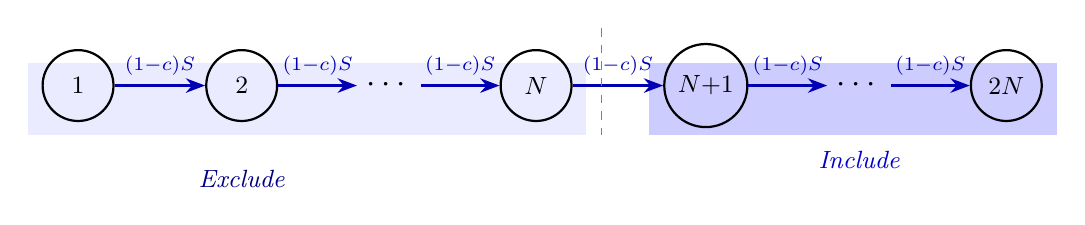
\begin{tikzpicture}[
  state/.style={circle, draw=black, thick, minimum size=0.9cm, font=\small},
  arr/.style={-{Stealth[length=7pt]}, thick, blue!70!black},
  node distance=1.15cm
]
\node[state] (s1) {$1$};
\node[state, right=of s1] (s2) {$2$};
\node[right=1cm of s2, font=\large] (d1) {$\cdots$};
\node[state, right=1cm of d1] (sN) {$N$};
\node[state, right=of sN] (sN1) {\small$N{+}1$};
\node[right=1cm of sN1, font=\large] (d2) {$\cdots$};
\node[state, right=1cm of d2] (s2N) {$2N$};

\draw[arr] (s1)  to node[above,font=\scriptsize]{$(1{-}c)S$} (s2);
\draw[arr] (s2)  to node[above,font=\scriptsize]{$(1{-}c)S$} (d1);
\draw[arr] (d1)  to node[above,font=\scriptsize]{$(1{-}c)S$} (sN);
\draw[arr] (sN)  to node[above,font=\scriptsize]{$(1{-}c)S$} (sN1);
\draw[arr] (sN1) to node[above,font=\scriptsize]{$(1{-}c)S$} (d2);
\draw[arr] (d2)  to node[above,font=\scriptsize]{$(1{-}c)S$} (s2N);

% Zone labels
\begin{scope}[on background layer]
  \fill[blue!8] ([xshift=-5pt,yshift=-18pt]s1.west) rectangle
               ([xshift=5pt, yshift=8pt] sN.east);
  \fill[blue!20] ([xshift=-5pt,yshift=-18pt]sN1.west) rectangle
               ([xshift=5pt, yshift=8pt] s2N.east);
\end{scope}
\node[below=14pt of s2, font=\small\itshape, text=blue!50!black] {Exclude};
\node[below=14pt of d2, font=\small\itshape, text=blue!80!black] {Include};

% Dashed separator
\draw[dashed, gray] ($(sN.north east)+(0.5,0.4)$) -- ($(sN.south east)+(0.5,-0.3)$);
\end{tikzpicture}
\caption{Chaîne de Markov de $v$ dans le cas IDENTITY sans bruit.
La chaîne ne progresse que vers \Inc{} ; aucune flèche retour n'existe.}
\label{fig:v_identity}
\end{figure}

\subsubsection*{Chaîne de l'automate $\vbar$}

\[
  \boxed{p^+_{\vbar} = 0, \qquad p^-_{\vbar} = (1-c)\cdot S + c\cdot \alpha.}
\]
Le scénario~1 applique \texttt{versExclude}$(S)$ à $\vbar$ (descend avec prob.\ $S$),
et le scénario~2 applique \texttt{versExclude}$(\alpha)$ (descend avec prob.\ $\alpha$).
Aucun scénario ne fait jamais monter $\vbar$.

\begin{figure}[h]
\centering
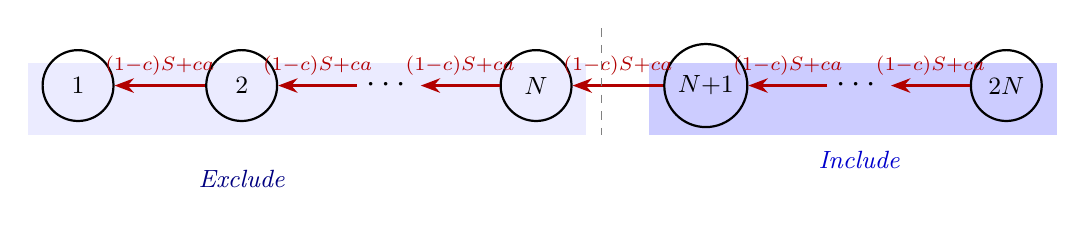
\begin{tikzpicture}[
  state/.style={circle, draw=black, thick, minimum size=0.9cm, font=\small},
  arr/.style={-{Stealth[length=7pt]}, thick, red!70!black},
  node distance=1.15cm
]
\node[state] (s1) {$1$};
\node[state, right=of s1] (s2) {$2$};
\node[right=1cm of s2, font=\large] (d1) {$\cdots$};
\node[state, right=1cm of d1] (sN) {$N$};
\node[state, right=of sN] (sN1) {\small$N{+}1$};
\node[right=1cm of sN1, font=\large] (d2) {$\cdots$};
\node[state, right=1cm of d2] (s2N) {$2N$};

\draw[arr] (s2)  to node[above,font=\scriptsize]{$(1{-}c)S{+}ca$} (s1);
\draw[arr] (d1)  to node[above,font=\scriptsize]{$(1{-}c)S{+}ca$} (s2);
\draw[arr] (sN)  to node[above,font=\scriptsize]{$(1{-}c)S{+}ca$} (d1);
\draw[arr] (sN1) to node[above,font=\scriptsize]{$(1{-}c)S{+}ca$} (sN);
\draw[arr] (d2)  to node[above,font=\scriptsize]{$(1{-}c)S{+}ca$} (sN1);
\draw[arr] (s2N) to node[above,font=\scriptsize]{$(1{-}c)S{+}ca$} (d2);

\begin{scope}[on background layer]
  \fill[blue!8]  ([xshift=-5pt,yshift=-18pt]s1.west)  rectangle ([xshift=5pt,yshift=8pt]sN.east);
  \fill[blue!20] ([xshift=-5pt,yshift=-18pt]sN1.west) rectangle ([xshift=5pt,yshift=8pt]s2N.east);
\end{scope}
\node[below=14pt of s2, font=\small\itshape, text=blue!50!black] {Exclude};
\node[below=14pt of d2, font=\small\itshape, text=blue!80!black] {Include};
\draw[dashed, gray] ($(sN.north east)+(0.5,0.4)$) -- ($(sN.south east)+(0.5,-0.3)$);
\end{tikzpicture}
\caption{Chaîne de Markov de $\vbar$ dans le cas IDENTITY sans bruit.
La chaîne ne progresse que vers \Exc{} ; aucune flèche retour n'existe.}
\label{fig:vbar_identity}
\end{figure}

\subsection{Théorème et preuve}

\begin{theorem}[Convergence IDENTITY, sans bruit]\label{thm:identity}
Dans le cas IDENTITY sans bruit ($y = x$, $c \in (0,1)$),
sous la règle à 4 cas avec $S,\alpha > 0$, pour toute configuration initiale
$(s_1^{(0)}, s_2^{(0)}) \in \{1,\ldots,2N\}^2$ :
\[
  v \longrightarrow \Inc \quad\text{et}\quad \vbar \longrightarrow \Exc \qquad
  \text{p.s.\ quand } t \to \infty,
\]
et par conséquent $C(x) \to x$, c'est-à-dire que la clause converge vers IDENTITY.
\end{theorem}

\begin{proof}
\textbf{Étape 1 : probabilités de transition de $v$.}
D'après le tableau des scénarios et le Lemme~\ref{lem:decoupling},
on a pour tout état intérieur de $v$, indépendamment de la configuration de $\vbar$ :
\[
  p^+_v = (1-c)\cdot S, \qquad p^-_v = 0.
\]

\textbf{Étape 2 : convergence de $v$ vers \Inc.}
Puisque $c < 1$ et $S > 0$, on a $p^+_v = (1-c)S > 0$.
Puisque $p^-_v = 0$, le Lemme~\ref{lem:convergence}(a) s'applique directement :
$s_1$ atteint l'état $2N$ en temps fini p.s.\ et y reste.  Donc $v \to \Inc$ p.s.

\textbf{Étape 3 : probabilités de transition de $\vbar$.}
De même, indépendamment de l'état de $v$ :
\[
  p^+_{\vbar} = 0, \qquad p^-_{\vbar} = (1-c)\cdot S + c\cdot \alpha.
\]

\textbf{Étape 4 : convergence de $\vbar$ vers \Exc.}
On a $p^-_{\vbar} = (1-c)S + ca \ge (1-c)S > 0$
(car $c < 1$ et $S > 0$).
Puisque $p^+_{\vbar} = 0$, le Lemme~\ref{lem:convergence}(b) s'applique :
$s_2$ atteint l'état $1$ en temps fini p.s.\ et y reste.  Donc $\vbar \to \Exc$ p.s.

\textbf{Étape 5 : conclusion.}
Les Étapes~2 et 4 sont établies \emph{indépendamment} l'une de l'autre
(grâce au Lemme~\ref{lem:decoupling}).  Pour tout $c \in (0,1)$, on a
simultanément $v \to \Inc$ et $\vbar \to \Exc$ p.s.,
quelle que soit la configuration initiale $(s_1^{(0)}, s_2^{(0)})$.
La clause converge vers $C(x) = \Inc(v) \wedge \Exc(\vbar) = x$,
soit la relation IDENTITY.
\end{proof}

\begin{remark}[Cas limites $c = 0$ et $c = 1$]
Si $c = 1$ (seuls des exemples $(1,1)$ arrivent), on a $p^+_v = (1-c)S = 0$ : $v$ n'évolue
plus et son état final dépend de l'initialisation.  La convergence vers IDENTITY n'est donc
\emph{pas} assurée pour $c = 1$ ($\vbar$, en revanche, converge toujours vers \Exc{}, car
$p^-_{\vbar} = ca > 0$).

À l'inverse, $c = 0$ \emph{ne} pose \emph{aucun} problème ici : $p^+_v = S > 0$ et
$p^-_{\vbar} = S > 0$, si bien que les deux automates convergent même en l'absence
d'exemples positifs $(1,1)$.  Cette asymétrie vient de ce que, sous la règle à 4 cas,
l'échantillon $(0,0)$ agit sur les \emph{deux} automates simultanément, alors que
$(1,1)$ n'agit que sur $\vbar$ (cf.\ tableau des scénarios ci-dessus).

Dans l'analyse originale de Zhang et al.\ \cite{zhang2021}, c'est au contraire $c=0$ qui
est dégénéré (et pour l'automate $\vbar$/TA2, qui cesse de bouger) : la dépendance du
retour de Type~II vis-à-vis de $C(x)$ couple les deux automates différemment de la règle
à 4 cas, ce qui déplace le point de dégénérescence.
\end{remark}

% ======================================================
\section{Cas NOT sans bruit}
% ======================================================

\subsection{Tableau des scénarios}

Dans le cas NOT ($y = 1-x$), seules deux réalisations de $(x,y)$ sont possibles :
$(0,1)$ avec probabilité $1-c$, et $(1,0)$ avec probabilité $c$.
Le tableau complet (huit scénarios) est le suivant.

\begin{center}
\renewcommand{\arraystretch}{1.35}
\begin{tabular}{llccll}
\toprule
Config.\ $(v,\vbar)$ & Scénario & $(x,y)$ & $C(x)$ & Action sur $v$ & Action sur $\vbar$ \\
\midrule
\multirow{2}{*}{$(E,E)$}
  & 1 & $(0,1)$ & $1$ & \texttt{versExclude}$(\alpha)$ & rien \\
  & 2 & $(1,0)$ & $1$ & \texttt{versExclude}$(S)$ & \texttt{versInclude}$(S)$ \\
\midrule
\multirow{2}{*}{$(E,I)$}
  & 3 & $(0,1)$ & $1$ & \texttt{versExclude}$(\alpha)$ & rien \\
  & 4 & $(1,0)$ & $0$ & \texttt{versExclude}$(S)$ & \texttt{versInclude}$(S)$ \\
\midrule
\multirow{2}{*}{$(I,E)$}
  & 5 & $(0,1)$ & $0$ & \texttt{versExclude}$(\alpha)$ & rien \\
  & 6 & $(1,0)$ & $1$ & \texttt{versExclude}$(S)$ & \texttt{versInclude}$(S)$ \\
\midrule
\multirow{2}{*}{$(I,I)$}
  & 7 & $(0,1)$ & $0$ & \texttt{versExclude}$(\alpha)$ & rien \\
  & 8 & $(1,0)$ & $0$ & \texttt{versExclude}$(S)$ & \texttt{versInclude}$(S)$ \\
\bottomrule
\end{tabular}
\end{center}

\medskip
\noindent
\textbf{Observation clé.}  Comme pour IDENTITY, la colonne $C(x)$ varie selon
la configuration (par exemple $C(0)=1$ pour $(E,E)$ mais $C(0)=0$ pour $(I,E)$),
mais les colonnes d'action sont \emph{constantes} pour chaque $(x,y)$.
Les huit scénarios se réduisent au tableau compact :

\begin{center}
\begin{tabular}{cccll}
\toprule
Scénario & $(x,y)$ & Probabilité & Action sur $v$ & Action sur $\vbar$ \\
\midrule
A & $(0,1)$ & $1-c$ & \texttt{versExclude}$(\alpha)$ & rien \\
B & $(1,0)$ & $c$   & \texttt{versExclude}$(S)$ & \texttt{versInclude}$(S)$ \\
\bottomrule
\end{tabular}
\end{center}

\subsection{Construction des chaînes de Markov}

\subsubsection*{Chaîne de l'automate $v$}

\[
  \boxed{p^+_v = 0, \qquad p^-_v = (1-c)\cdot \alpha + c\cdot S.}
\]
Le scénario~1 (prob.\ $1-c$) applique \texttt{versExclude}$(\alpha)$ à $v$
(descend avec prob.\ $\alpha$).
Le scénario~2 (prob.\ $c$) applique \texttt{versExclude}$(S)$ à $v$
(descend avec prob.\ $S$).
Aucun scénario ne fait jamais monter $v$.

\begin{figure}[h]
\centering
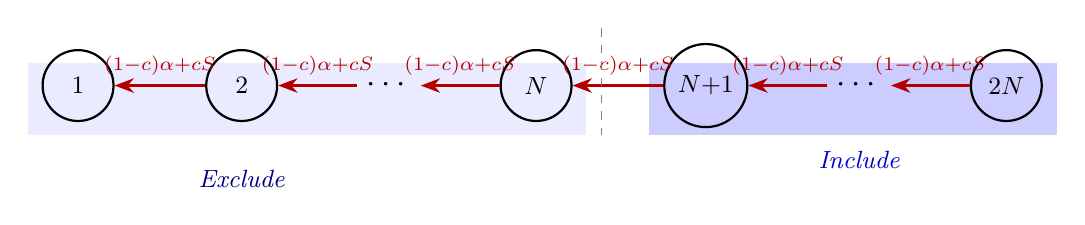
\begin{tikzpicture}[
  state/.style={circle, draw=black, thick, minimum size=0.9cm, font=\small},
  arr/.style={-{Stealth[length=7pt]}, thick, red!70!black},
  node distance=1.15cm
]
\node[state] (s1) {$1$};
\node[state, right=of s1] (s2) {$2$};
\node[right=1cm of s2, font=\large] (d1) {$\cdots$};
\node[state, right=1cm of d1] (sN) {$N$};
\node[state, right=of sN] (sN1) {\small$N{+}1$};
\node[right=1cm of sN1, font=\large] (d2) {$\cdots$};
\node[state, right=1cm of d2] (s2N) {$2N$};

\draw[arr] (s2)  to node[above,font=\scriptsize]{$(1{-}c)\alpha{+}cS$} (s1);
\draw[arr] (d1)  to node[above,font=\scriptsize]{$(1{-}c)\alpha{+}cS$} (s2);
\draw[arr] (sN)  to node[above,font=\scriptsize]{$(1{-}c)\alpha{+}cS$} (d1);
\draw[arr] (sN1) to node[above,font=\scriptsize]{$(1{-}c)\alpha{+}cS$} (sN);
\draw[arr] (d2)  to node[above,font=\scriptsize]{$(1{-}c)\alpha{+}cS$} (sN1);
\draw[arr] (s2N) to node[above,font=\scriptsize]{$(1{-}c)\alpha{+}cS$} (d2);

\begin{scope}[on background layer]
  \fill[blue!8]  ([xshift=-5pt,yshift=-18pt]s1.west)  rectangle ([xshift=5pt,yshift=8pt]sN.east);
  \fill[blue!20] ([xshift=-5pt,yshift=-18pt]sN1.west) rectangle ([xshift=5pt,yshift=8pt]s2N.east);
\end{scope}
\node[below=14pt of s2, font=\small\itshape, text=blue!50!black] {Exclude};
\node[below=14pt of d2, font=\small\itshape, text=blue!80!black] {Include};
\draw[dashed, gray] ($(sN.north east)+(0.5,0.4)$) -- ($(sN.south east)+(0.5,-0.3)$);
\end{tikzpicture}
\caption{Chaîne de Markov de $v$ dans le cas NOT sans bruit.
La chaîne ne progresse que vers \Exc{} ; aucune flèche retour n'existe.}
\label{fig:v_not}
\end{figure}

\subsubsection*{Chaîne de l'automate $\vbar$}

\[
  \boxed{p^+_{\vbar} = c\cdot S, \qquad p^-_{\vbar} = 0.}
\]
Seul le scénario~2 (prob.\ $c$) agit sur $\vbar$ : il applique \texttt{versInclude}$(S)$,
déplaçant $\vbar$ vers la droite avec probabilité $S$.  Le scénario~1 n'agit pas sur $\vbar$.
Aucun scénario ne fait jamais descendre $\vbar$.

\begin{figure}[h]
\centering
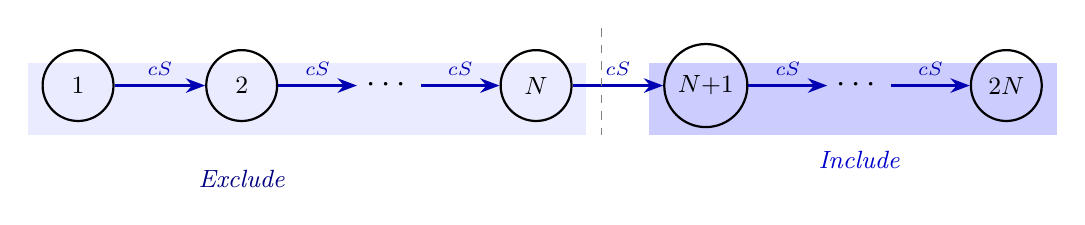
\begin{tikzpicture}[
  state/.style={circle, draw=black, thick, minimum size=0.9cm, font=\small},
  arr/.style={-{Stealth[length=7pt]}, thick, blue!70!black},
  node distance=1.15cm
]
\node[state] (s1) {$1$};
\node[state, right=of s1] (s2) {$2$};
\node[right=1cm of s2, font=\large] (d1) {$\cdots$};
\node[state, right=1cm of d1] (sN) {$N$};
\node[state, right=of sN] (sN1) {\small$N{+}1$};
\node[right=1cm of sN1, font=\large] (d2) {$\cdots$};
\node[state, right=1cm of d2] (s2N) {$2N$};

\draw[arr] (s1)  to node[above,font=\scriptsize]{$cS$} (s2);
\draw[arr] (s2)  to node[above,font=\scriptsize]{$cS$} (d1);
\draw[arr] (d1)  to node[above,font=\scriptsize]{$cS$} (sN);
\draw[arr] (sN)  to node[above,font=\scriptsize]{$cS$} (sN1);
\draw[arr] (sN1) to node[above,font=\scriptsize]{$cS$} (d2);
\draw[arr] (d2)  to node[above,font=\scriptsize]{$cS$} (s2N);

\begin{scope}[on background layer]
  \fill[blue!8]  ([xshift=-5pt,yshift=-18pt]s1.west)  rectangle ([xshift=5pt,yshift=8pt]sN.east);
  \fill[blue!20] ([xshift=-5pt,yshift=-18pt]sN1.west) rectangle ([xshift=5pt,yshift=8pt]s2N.east);
\end{scope}
\node[below=14pt of s2, font=\small\itshape, text=blue!50!black] {Exclude};
\node[below=14pt of d2, font=\small\itshape, text=blue!80!black] {Include};
\draw[dashed, gray] ($(sN.north east)+(0.5,0.4)$) -- ($(sN.south east)+(0.5,-0.3)$);
\end{tikzpicture}
\caption{Chaîne de Markov de $\vbar$ dans le cas NOT sans bruit.
La chaîne ne progresse que vers \Inc{} ; aucune flèche retour n'existe.}
\label{fig:vbar_not}
\end{figure}

\subsection{Théorème et preuve}

\begin{theorem}[Convergence NOT, sans bruit]\label{thm:not}
Dans le cas NOT sans bruit ($y = 1-x$, $c \in (0,1)$),
sous la règle à 4 cas avec $S,\alpha > 0$, pour toute configuration initiale
$(s_1^{(0)}, s_2^{(0)}) \in \{1,\ldots,2N\}^2$ :
\[
  v \longrightarrow \Exc \quad\text{et}\quad \vbar \longrightarrow \Inc \qquad
  \text{p.s.\ quand } t \to \infty,
\]
et par conséquent $C(x) \to \neg x$, c'est-à-dire que la clause converge vers NOT.
\end{theorem}

\begin{proof}
\textbf{Étape 1 : probabilités de transition de $v$.}
D'après le tableau des scénarios et le Lemme~\ref{lem:decoupling} :
\[
  p^+_v = 0, \qquad p^-_v = (1-c)\cdot \alpha + c\cdot S.
\]

\textbf{Étape 2 : convergence de $v$ vers \Exc.}
On a $p^-_v = (1-c)\alpha + cS \ge cS > 0$ (car $c > 0$ et $S > 0$).
De plus, $(1-c)\alpha \ge 0$ renforce ce terme quand $c < 1$.
Puisque $p^+_v = 0$, le Lemme~\ref{lem:convergence}(b) s'applique :
$s_1$ atteint l'état $1$ en temps fini p.s.\ et y reste.  Donc $v \to \Exc$ p.s.

\textbf{Étape 3 : probabilités de transition de $\vbar$.}
De même :
\[
  p^+_{\vbar} = c\cdot S, \qquad p^-_{\vbar} = 0.
\]

\textbf{Étape 4 : convergence de $\vbar$ vers \Inc.}
Puisque $c > 0$ et $S > 0$, on a $p^+_{\vbar} = cS > 0$.
Puisque $p^-_{\vbar} = 0$, le Lemme~\ref{lem:convergence}(a) s'applique :
$s_2$ atteint l'état $2N$ en temps fini p.s.\ et y reste.  Donc $\vbar \to \Inc$ p.s.

\textbf{Étape 5 : conclusion.}
De même que pour IDENTITY, les Étapes~2 et 4 sont établies indépendamment
(Lemme~\ref{lem:decoupling}).  Pour tout $c \in (0,1)$, on a simultanément
$v \to \Exc$ et $\vbar \to \Inc$ p.s.  La clause converge vers
$C(x) = \Exc(v) \wedge \Inc(\vbar) = \neg x$, soit la relation NOT.
\end{proof}

\begin{remark}[Cas limites $c = 0$ et $c = 1$]
Si $c = 1$ (seuls des exemples $(1,0)$ arrivent), la convergence de $v$ vers \Exc{}
reste garantie ($p^-_v = S > 0$), et $p^+_{\vbar} = S > 0$ avec $p^-_{\vbar} = 0$,
donc $\vbar \to \Inc$ également --- la convergence NOT est donc garantie
pour $c = 1$, par symétrie exacte avec le cas IDENTITY lorsque $c = 0$.

À l'inverse, si $c = 0$ (seuls des exemples $(0,1)$ arrivent), $p^+_{\vbar} = cS = 0$ :
$\vbar$ n'évolue plus et la convergence vers NOT n'est \emph{pas} assurée pour $c=0$,
par symétrie exacte avec le cas dégénéré $c=1$ d'IDENTITY.
\end{remark}

% ======================================================
\section{Synthèse du cas sans bruit}\label{sec:synthese_snb}
% ======================================================

\subsection{Tableau récapitulatif}

\begin{center}
\renewcommand{\arraystretch}{1.4}
\begin{tabular}{lcccc}
\toprule
Opérateur & $p^+_v$ & $p^-_v$ & $p^+_{\vbar}$ & $p^-_{\vbar}$ \\
\midrule
IDENTITY ($y=x$)   & $(1-c)S$ & $0$ & $0$ & $(1-c)S + ca$ \\
NOT ($y=1-x$)      & $0$ & $(1-c)\alpha + cS$ & $cS$ & $0$ \\
\bottomrule
\end{tabular}
\end{center}

\begin{center}
\renewcommand{\arraystretch}{1.4}
\begin{tabular}{lccc}
\toprule
Opérateur & Condition & Résultat ($v$, $\vbar$) & $C(x)$ \\
\midrule
IDENTITY & $c \in (0,1)$ & $(\Inc,\; \Exc)$ & $x$ \\
NOT      & $c \in (0,1)$ & $(\Exc,\; \Inc)$ & $\neg x$ \\
\bottomrule
\end{tabular}
\end{center}

\subsection{Symétrie IDENTITY / NOT}

La règle à 4 cas est \textbf{parfaitement symétrique} entre les deux opérateurs.
En échangeant les rôles de $x$ et $\neg x$ (et donc de $v$ et $\vbar$),
et en remplaçant $c$ par $1-c$, on passe exactement du cas IDENTITY au cas NOT.
Cette symétrie est visible dans les probabilités de transition :
\begin{align*}
  p^+_v(\text{IDENTITY}) &= (1-c)S \;\leftrightarrow\; p^+_{\vbar}(\text{NOT}) = cS, \\
  p^-_{\vbar}(\text{IDENTITY}) &= (1-c)S + ca \;\leftrightarrow\; p^-_v(\text{NOT}) = cS + (1-c)\alpha.
\end{align*}

\subsection{Comparaison avec la TM originale}

\begin{center}
\renewcommand{\arraystretch}{1.3}
\begin{tabular}{p{6cm}p{6cm}}
\toprule
\textbf{Règle à 4 cas (ce travail)} & \textbf{TM originale (Zhang et al., 2021)} \\
\midrule
Mise à jour indépendante de $C(x)$ & Mise à jour dépend de $C(x)$ \\
\addlinespace
2 chaînes de Markov indépendantes & 4 chaînes de Markov couplées \\
\addlinespace
Convergence p.s.\ dès $c \in (0,1)$, sans condition sur $N$ & Convergence pour tout $N \ge 1$ (Remarque~1 dans \cite{zhang2021}) \\
\addlinespace
Cas $c=1$ dégénéré pour IDENTITY (pour $v$) & Cas $c=0$ dégénéré pour $\vbar$ \\
\addlinespace
Preuve en 5 étapes directes & Preuve par analyse quasi-stationnaire et chaînes conditionnelles \\
\bottomrule
\end{tabular}
\end{center}

% ======================================================
\section{Cas avec bruit}
% ======================================================

\subsection{Modèle de bruit}\label{sec:modele_bruit}

On suppose maintenant que le label $y$ est \textbf{stochastique}.  On caractérise le canal
de bruit par deux paramètres :
\[
  a = P(y=1 \mid x=1), \qquad b = P(y=1 \mid x=0), \qquad a,b \in (0,1),\; a \ne b.
\]
Le cas sans bruit est le cas limite : $(a,b)\to(1,0)$ pour IDENTITY et $(a,b)\to(0,1)$ pour NOT.
On conserve la notation $c = P(x=1) \in (0,1)$ du cas sans bruit.

Avec le bruit, les quatre combinaisons $(x,y)$ deviennent toutes possibles.
La règle à 4 cas s'applique de la même façon (Lemme~\ref{lem:decoupling} toujours valide),
mais les fréquences relatives des cas changent :

\begin{center}
\renewcommand{\arraystretch}{1.3}
\begin{tabular}{ccll}
\toprule
$(x,y)$ & Probabilité & Action sur $v$ & Action sur $\vbar$ \\
\midrule
$(0,0)$ & $(1-c)(1-b)$  & \texttt{versInclude}$(S)$ & \texttt{versExclude}$(S)$ \\
$(0,1)$ & $(1-c)b$      & \texttt{versExclude}$(\alpha)$ & rien \\
$(1,0)$ & $c(1-a)$     & \texttt{versExclude}$(S)$ & \texttt{versInclude}$(S)$ \\
$(1,1)$ & $ca$         & rien & \texttt{versExclude}$(\alpha)$ \\
\bottomrule
\end{tabular}
\end{center}

\medskip
Dorénavant $p^+ > 0$ \emph{et} $p^- > 0$ pour chaque automate : les chaînes de Markov sont
\textbf{bidirectionnelles} (Figure~\ref{fig:chaine_bruit}), et le Lemme~\ref{lem:convergence}
(absorption p.s.) ne s'applique plus.  On va montrer qu'elles sont cependant \emph{ergodiques},
et que leur distribution stationnaire se concentre sur la région correcte sous une condition
sur $S$.

\begin{figure}[h]
\centering
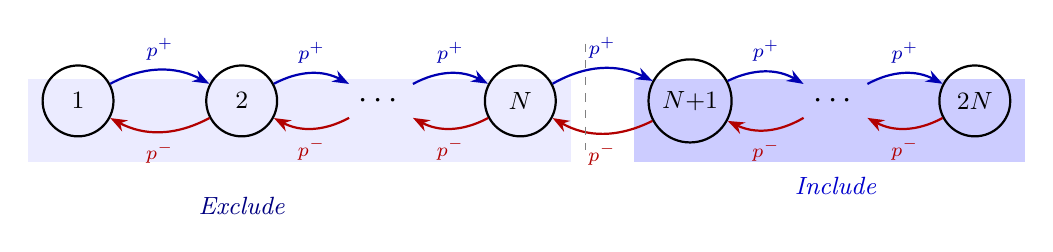
\begin{tikzpicture}[
  state/.style={circle, draw=black, thick, minimum size=0.9cm, font=\small},
  node distance=1.15cm
]
\node[state] (s1) {$1$};
\node[state, right=of s1] (s2) {$2$};
\node[right=0.9cm of s2, font=\large] (d1) {$\cdots$};
\node[state, right=0.9cm of d1] (sN) {$N$};
\node[state, right=of sN] (sN1) {\small$N{+}1$};
\node[right=0.9cm of sN1, font=\large] (d2) {$\cdots$};
\node[state, right=0.9cm of d2] (s2N) {$2N$};

\draw[-{Stealth[length=6pt]}, thick, blue!70!black]
  (s1) to[bend left=28] node[above,font=\scriptsize]{$p^+$} (s2);
\draw[-{Stealth[length=6pt]}, thick, blue!70!black]
  (s2) to[bend left=28] node[above,font=\scriptsize]{$p^+$} (d1);
\draw[-{Stealth[length=6pt]}, thick, blue!70!black]
  (d1) to[bend left=28] node[above,font=\scriptsize]{$p^+$} (sN);
\draw[-{Stealth[length=6pt]}, thick, blue!70!black]
  (sN) to[bend left=28] node[above,font=\scriptsize]{$p^+$} (sN1);
\draw[-{Stealth[length=6pt]}, thick, blue!70!black]
  (sN1) to[bend left=28] node[above,font=\scriptsize]{$p^+$} (d2);
\draw[-{Stealth[length=6pt]}, thick, blue!70!black]
  (d2) to[bend left=28] node[above,font=\scriptsize]{$p^+$} (s2N);

\draw[-{Stealth[length=6pt]}, thick, red!70!black]
  (s2) to[bend left=28] node[below,font=\scriptsize]{$p^-$} (s1);
\draw[-{Stealth[length=6pt]}, thick, red!70!black]
  (d1) to[bend left=28] node[below,font=\scriptsize]{$p^-$} (s2);
\draw[-{Stealth[length=6pt]}, thick, red!70!black]
  (sN) to[bend left=28] node[below,font=\scriptsize]{$p^-$} (d1);
\draw[-{Stealth[length=6pt]}, thick, red!70!black]
  (sN1) to[bend left=28] node[below,font=\scriptsize]{$p^-$} (sN);
\draw[-{Stealth[length=6pt]}, thick, red!70!black]
  (d2) to[bend left=28] node[below,font=\scriptsize]{$p^-$} (sN1);
\draw[-{Stealth[length=6pt]}, thick, red!70!black]
  (s2N) to[bend left=28] node[below,font=\scriptsize]{$p^-$} (d2);

\begin{scope}[on background layer]
  \fill[blue!8]  ([xshift=-5pt,yshift=-22pt]s1.west)  rectangle ([xshift=5pt,yshift=8pt]sN.east);
  \fill[blue!20] ([xshift=-5pt,yshift=-22pt]sN1.west) rectangle ([xshift=5pt,yshift=8pt]s2N.east);
\end{scope}
\node[below=18pt of s2, font=\small\itshape, text=blue!50!black] {Exclude};
\node[below=18pt of d2, font=\small\itshape, text=blue!80!black] {Include};
\draw[dashed, gray] ($(sN.north east)+(0.5,0.4)$) -- ($(sN.south east)+(0.5,-0.3)$);
\end{tikzpicture}
\caption{Chaîne de Markov bidirectionnelle dans le cas bruité : flèches bleues ($p^+$) vers
\Inc{} et flèches rouges ($p^-$) vers \Exc.  La distribution stationnaire est géométrique
de raison $\rho = p^+/p^-$.}
\label{fig:chaine_bruit}
\end{figure}

% -------------------------------------------------------
\subsection{Rappels : deux théorèmes classiques}
% -------------------------------------------------------

La preuve du lemme suivant repose sur deux résultats standards de la théorie des chaînes
de Markov, que l'on rappelle ici pour être explicite.

\begin{theorem}[Théorème ergodique, chaîne finie {\normalfont\cite{norris1997}}]\label{thm:ergo}
Toute chaîne de Markov à espace d'états fini, \emph{irréductible} et \emph{apériodique},
admet une unique distribution stationnaire $\pi$, et pour tout état initial $k_0$ :
\[
  P(X_t = k \mid X_0 = k_0) \;\xrightarrow{t\to\infty}\; \pi(k) \qquad \forall\, k.
\]
\end{theorem}

\begin{theorem}[Bilan détaillé {\normalfont\cite{norris1997}}]\label{thm:balance}
Si une distribution $\pi$ sur les états d'une chaîne de Markov vérifie la condition de
\emph{bilan détaillé} :
\[
  \pi(i)\,p_{ij} = \pi(j)\,p_{ji} \qquad \forall\, i,j,
\]
alors $\pi$ est une distribution stationnaire de cette chaîne.
\end{theorem}

% -------------------------------------------------------
\subsection{Lemme de convergence ergodique}
% -------------------------------------------------------

\begin{lemma}[Chaîne bidirectionnelle]\label{lem:ergodique}
Soit une chaîne de Markov homogène sur $\{1,\ldots,2N\}$ avec, pour tout état intérieur
$k\in\{2,\ldots,2N-1\}$ :
\[
  p(k\to k+1) = p^+ > 0, \quad p(k\to k-1) = p^- > 0, \quad p(k\to k) = 1-p^+-p^-,
\]
et aux bords : $p(1\to 2)=p^+$, $p(2N\to 2N-1)=p^-$ (réflexion).
Posons $\rho = p^+/p^-$.

La chaîne est \textbf{ergodique} et sa distribution stationnaire $\pi$ satisfait
$\pi(k) \propto \rho^k$.  La probabilité stationnaire d'être dans $\Inc = \{N+1,\ldots,2N\}$ est :
\[
  \boxed{\pi(\Inc) = \frac{\rho^N}{\rho^N + 1}.}
\]
\begin{itemize}
  \item Si $\rho > 1$ : $\pi(\Inc) > \tfrac{1}{2}$ et $1-\pi(\Inc) = \dfrac{1}{\rho^N+1} \le \rho^{-N} \xrightarrow{N\to\infty} 0$ exponentiellement.
  \item Si $\rho < 1$ : $\pi(\Exc) = \dfrac{1}{\rho^N+1} \xrightarrow{N\to\infty} 1$.
\end{itemize}
\end{lemma}

\begin{proof}

\medskip
\textbf{Étape 1 : la chaîne est ergodique (Théorème~\ref{thm:ergo}).}

\emph{Irréductibilité.}  Pour tout $i < j$, on peut aller de $i$ à $j$ en $j-i$ pas vers
la droite, chacun de probabilité $p^+ > 0$.  De même on va de $j$ à $i$ en $j-i$ pas vers
la gauche.  Donc tous les états communiquent.

\emph{Apériodicité.}  Tout état intérieur vérifie $p(k\to k) = 1-p^+-p^- > 0$
(on choisit $p^++p^- \le 1$), donc la chaîne peut rester sur place en un pas : la période est~$1$.

Par le Théorème~\ref{thm:ergo}, la chaîne admet une unique distribution stationnaire $\pi$,
et $P(X_t=k\mid X_0=k_0)\to\pi(k)$ pour tout $k_0$.

\medskip
\textbf{Étape 2 : distribution stationnaire par bilan détaillé (Théorème~\ref{thm:balance}).}

\paragraph{Qu'est-ce que le bilan détaillé ?}
Pour une chaîne de Markov de matrice de transition $(p_{ij})$, une distribution $\pi$ est
\emph{stationnaire} si $\pi P = \pi$, c'est-à-dire si pour chaque état $j$, le flux de
probabilité \emph{entrant} égale le flux \emph{sortant} : $\sum_i \pi(i)p_{ij} = \pi(j)
= \pi(j)\sum_i p_{ji}$.  C'est un bilan \emph{global}, sommé sur tous les états $i$.

Le \textbf{bilan détaillé} est une condition plus forte, et plus simple à vérifier : on
exige que ce bilan soit nul \emph{entre chaque paire d'états prise séparément}, et non
plus seulement en moyenne sur tous les états :
\[
  \pi(i)\,p_{ij} = \pi(j)\,p_{ji} \qquad \text{pour tout } i,j.
\]
Interprétation : si l'on imagine une grande population de copies indépendantes de la
chaîne, réparties selon $\pi$, alors $\pi(i)p_{ij}$ est la quantité de probabilité qui
« s'écoule » de $i$ vers $j$ à chaque pas de temps.  Le bilan détaillé affirme que ce
flux est \emph{exactement compensé}, paire par paire, par le flux retour de $j$ vers
$i$ : aucun courant net ne circule entre deux états quelconques.  C'est strictement
plus fort que la stationnarité (qui n'annule que le bilan \emph{total}), mais cela
implique la stationnarité (Théorème~\ref{thm:balance}) : en sommant sur $i$,
$\sum_i \pi(i)p_{ij} = \sum_i \pi(j)p_{ji} = \pi(j)\sum_i p_{ji} = \pi(j)$.

\paragraph{Ce qu'on utilise ici.}
Pour notre chaîne, $p_{ij}=0$ dès que $|i-j|>1$ (chaîne de naissance et de mort) : le
bilan détaillé est donc \emph{automatiquement} vérifié (trivialement, $0=0$) pour toute
paire non adjacente.  Il ne reste à vérifier que les paires voisines $(k,k+1)$, pour
lesquelles les seules transitions non nulles sont $p_{k,k+1}=p^+$ et $p_{k+1,k}=p^-$.

\paragraph{D'où vient la forme $\rho^k$ ?}
Plutôt que de deviner la forme de $\pi$, on peut la \emph{dériver} directement de la
condition de bilan détaillé.  Pour $k=1,\ldots,2N-1$ :
\[
  \pi(k)\,p^+ = \pi(k+1)\,p^-
  \quad\Longrightarrow\quad
  \frac{\pi(k+1)}{\pi(k)} = \frac{p^+}{p^-} = \rho.
\]
Ce rapport est \emph{constant} (le même $\rho$ pour tout $k$), car $p^+$ et $p^-$ ne
dépendent pas de l'état $k$ : ce sont des constantes fixées par les hypothèses du lemme.
Par récurrence immédiate :
\[
  \pi(k) = \pi(1)\cdot \rho^{k-1} = \underbrace{\left(\frac{\pi(1)}{\rho}\right)}_{=:\,C} \cdot \rho^k,
\]
ce qui explique l'apparition de la forme géométrique $\pi(k)=C\rho^k$.  On vérifie
ensuite que cette famille satisfait bien le bilan détaillé pour toute paire adjacente
$k$, $k+1$ :
\[
  \pi(k)\cdot p^+ \;=\; C\rho^k\cdot p^+
  \qquad \text{et} \qquad
  \pi(k+1)\cdot p^- \;=\; C\rho^{k+1}\cdot p^- = C\rho^k \cdot \rho p^- = C\rho^k \cdot p^+.
\]
Les deux membres sont égaux, donc le bilan détaillé est satisfait.
Par le Théorème~\ref{thm:balance}, $\pi(k) = C\,\rho^k$ est \textbf{stationnaire}.
La constante $C$ est fixée par la normalisation $\sum_{k=1}^{2N}\pi(k)=1$ :
\[
  C \sum_{k=1}^{2N}\rho^k = C\,\frac{\rho(\rho^{2N}-1)}{\rho-1} = 1
  \quad\Longrightarrow\quad
  C = \frac{\rho-1}{\rho(\rho^{2N}-1)}.
\]

\medskip
\textbf{Étape 3 : calcul de $\pi(\Inc)$ par série géométrique.}

\begin{align*}
  \pi(\Inc) &= \sum_{k=N+1}^{2N} C\,\rho^k
              = C\,\rho^{N+1}\,\frac{\rho^N - 1}{\rho - 1}\\[6pt]
            &= \frac{\rho-1}{\rho(\rho^{2N}-1)}\cdot\frac{\rho^{N+1}(\rho^N-1)}{\rho-1}
             = \frac{\rho^N(\rho^N-1)}{\rho^{2N}-1}
             = \frac{\rho^N(\rho^N-1)}{(\rho^N-1)(\rho^N+1)}
             = \frac{\rho^N}{\rho^N+1}.
\end{align*}

\medskip
\textbf{Étape 4 : comportement en $N$.}

Si $\rho > 1$ : $\rho^N \to +\infty$, donc $\pi(\Inc) = \rho^N/(\rho^N+1) \to 1$.
La vitesse de convergence est exponentielle :
\[
  1 - \pi(\Inc) = \frac{1}{\rho^N+1} \;\le\; \rho^{-N}.
\]
Si $\rho < 1$ : $\rho^N \to 0$, donc $\pi(\Inc)\to 0$ et $\pi(\Exc) = 1-\pi(\Inc)\to 1$.
\end{proof}

% -------------------------------------------------------
\subsection{Vitesse de convergence : saturation et compromis entre $v$ et $\vbar$}\label{sec:vitesse_convergence}
% -------------------------------------------------------

Le Lemme~\ref{lem:ergodique} affirme que $\pi(\Inc)\to1$ quand $\rho>1$, mais la borne
$1-\pi(\Inc)\le\rho^{-N}$ qu'il fournit permet d'aller plus loin : quantifier
\emph{combien} d'états $N$ sont nécessaires, et comment ce nombre dépend du paramètre
$S$ choisi pour la règle d'apprentissage.

\subsubsection*{Nombre d'états nécessaire pour une précision donnée}

Fixons une tolérance d'erreur $\varepsilon \in (0,1)$ et demandons $1-\pi(\Inc)\le\varepsilon$.
Comme $1-\pi(\Inc)\le\rho^{-N}$ (Lemme~\ref{lem:ergodique}), il suffit que $\rho^{-N}\le\varepsilon$.
En prenant le logarithme (et en divisant par $\ln\rho>0$, qui est positif puisque $\rho>1$,
ce qui ne renverse pas le sens de l'inégalité) :
\[
  \boxed{N \;\ge\; \frac{\ln(1/\varepsilon)}{\ln\rho}.}
\]
C'est une condition \emph{suffisante} : elle fournit une règle de dimensionnement
directe pour le nombre d'états $2N$ de l'automate, en fonction de la précision visée
$\varepsilon$ et du paramètre $\rho$ du modèle.

\subsubsection*{Ralentissement critique près de $\rho = 1$}

Posons $\rho = 1+\delta$ avec $\delta \to 0^+$. Le développement de Taylor
$\ln(1+\delta) \approx \delta$ donne :
\[
  N \;\gtrsim\; \frac{\ln(1/\varepsilon)}{\delta}.
\]
Le nombre d'états nécessaire explose comme $1/\delta$ lorsque $\rho$ s'approche de $1$ :
diviser par deux l'écart $\delta$ oblige à \emph{doubler} $N$. C'est un phénomène de
ralentissement critique, semblable à celui observé près du seuil de transitivité dans
de nombreuses chaînes de Markov : plus le signal (l'écart de $\rho$ au-dessus de $1$)
est faible, plus la mémoire de l'automate doit être grande pour le détecter de façon
fiable.

\subsubsection*{$\rho$ ne croît pas indéfiniment avec $S$}

Pour $v$ comme pour $\vbar$, les probabilités de transition ont la forme
$p^+(S)=AS$ et $p^-(S)=BS+D$ (constantes $A,B,D>0$ ne dépendant que de $a,b,c$,
calculées ci-dessous). Le rapport $\rho(S)=AS/(BS+D)$ est alors :
\begin{itemize}
  \item \textbf{croissant} en $S$ : plus $S$ est grand, plus $\rho$ est grand,
  donc plus la convergence est rapide (formule de $N(\varepsilon)$ ci-dessus) ;
  \item \textbf{plafonné} : en divisant haut et bas par $S$,
  $\rho(S)=\dfrac{A}{B+D/S} \xrightarrow[S\to\infty]{} \dfrac{A}{B}$, une valeur
  \textbf{finie}.
\end{itemize}
Augmenter $S$ aide donc toujours, mais seulement jusqu'à un certain point : à bruit
fixé, il existe une vitesse de convergence maximale qu'aucun choix de $S$ ne peut
dépasser.

\subsubsection*{Application à $v$ et $\vbar$ : deux plafonds réciproques}

\paragraph{D'où viennent $p^+_v$, $p^-_v$, $p^+_{\vbar}$, $p^-_{\vbar}$ ?}
Reprenons le tableau des quatre cas $(x,y)$ de la Section~\ref{sec:modele_bruit} (rappel :
les probabilités s'obtiennent par $P(x,y)=P(x)\cdot P(y\mid x)$, avec $P(x{=}1)=c$,
$P(y{=}1\mid x{=}1)=a$, $P(y{=}1\mid x{=}0)=b$) :

\begin{center}
\renewcommand{\arraystretch}{1.3}
\begin{tabular}{ccll}
\toprule
$(x,y)$ & Probabilité & Action sur $v$ & Action sur $\vbar$ \\
\midrule
$(0,0)$ & $(1-c)(1-b)$  & \texttt{versInclude}$(S)$ & \texttt{versExclude}$(S)$ \\
$(0,1)$ & $(1-c)b$      & \texttt{versExclude}$(\alpha)$ & rien \\
$(1,0)$ & $c(1-a)$     & \texttt{versExclude}$(S)$ & \texttt{versInclude}$(S)$ \\
$(1,1)$ & $ca$         & rien & \texttt{versExclude}$(\alpha)$ \\
\bottomrule
\end{tabular}
\end{center}

Exactement comme dans le cas sans bruit (Lemme~\ref{lem:decoupling}), on obtient $p^+_v$
en additionnant les probabilités des lignes qui poussent $v$ vers \Inc, et $p^-_v$ en
additionnant celles qui le poussent vers \Exc{} :
\begin{itemize}
  \item \textbf{Vers \Inc{} pour $v$} : une seule ligne, $(0,0)$, probabilité
  $(1-c)(1-b)$, succès $S$ $\Rightarrow$ $p^+_v = (1-c)(1-b)\,S$.
  \item \textbf{Vers \Exc{} pour $v$} : deux lignes, $(0,1)$ [probabilité $(1-c)b$,
  succès $\alpha$] et $(1,0)$ [probabilité $c(1-a)$, succès $S$]
  $\Rightarrow$ $p^-_v = (1-c)b\,\alpha + c(1-a)\,S$.
  \item \textbf{Vers \Inc{} pour $\vbar$} : une seule ligne, $(1,0)$, probabilité
  $c(1-a)$, succès $S$ $\Rightarrow$ $p^+_{\vbar} = c(1-a)\,S$.
  \item \textbf{Vers \Exc{} pour $\vbar$} : deux lignes, $(0,0)$ [probabilité
  $(1-c)(1-b)$, succès $S$] et $(1,1)$ [probabilité $ca$, succès $\alpha$]
  $\Rightarrow$ $p^-_{\vbar} = (1-c)(1-b)\,S + ca\,\alpha$.
\end{itemize}
En résumé :
\begin{align}
  p^+_v &= (1-c)(1-b)\,S, &
  p^-_v &= (1-c)b\,\alpha + c(1-a)\,S; \label{eq:pv_id}\\[4pt]
  p^+_{\vbar} &= c(1-a)\,S, &
  p^-_{\vbar} &= (1-c)(1-b)\,S + ca\,\alpha. \label{eq:pvbar_id}
\end{align}
On note $\rho_v = p^+_v/p^-_v$ et $\rho_{\vbar} = p^+_{\vbar}/p^-_{\vbar}$. Les deux sont
bien de la forme $AS/(BS+D)$ vue ci-dessus, donc strictement croissantes en $S$, de
plafonds respectifs :
\[
  \rho_v^{\max} = \frac{(1-c)(1-b)}{c(1-a)},
  \qquad
  \rho_{\vbar}^{\max} = \frac{c(1-a)}{(1-c)(1-b)}.
\]
On remarque immédiatement que :
\[
  \boxed{\rho_v^{\max} \cdot \rho_{\vbar}^{\max} = 1.}
\]
Les deux plafonds sont \textbf{réciproques}. Cette identité explique, d'un seul coup,
un fait qui apparaîtra séparément dans les deux sections suivantes : par définition de
$\Delta=(1-c)(1-b)-c(1-a)$, on a $\Delta>0 \iff \rho_v^{\max}>1 \iff
\rho_{\vbar}^{\max}<1$ — l'un des deux plafonds ne peut dépasser $1$ que si l'autre
tombe en-dessous. C'est la raison structurelle pour laquelle, dans le
Théorème~\ref{thm:identity_bruit}, la convergence de $\vbar$ est
\emph{inconditionnelle} dès que $\Delta>0$, alors que celle de $v$ exige une condition
explicite sur $S$ : $\vbar$ se trouve déjà, pour tout $S$, dans la zone $\rho_{\vbar}<1$,
alors que $v$ doit \emph{atteindre} la zone $\rho_v>1$ en augmentant $S$ suffisamment.

\textbf{Le compromis caché.} Puisque $\rho_{\vbar}(S)$ est elle aussi strictement
croissante (vers son plafond $\rho_{\vbar}^{\max}<1$), augmenter $S$ accélère la
convergence de $v$ vers \Inc{} mais \emph{ralentit} celle de $\vbar$ vers \Exc{} (sans
jamais compromettre cette dernière, puisqu'elle reste sous $1$). Choisir $S$ n'est donc
pas seulement une question de seuil à dépasser (voir la condition sur $S$ dans la
section suivante) : c'est aussi un compromis entre les vitesses de convergence des deux
automates.

\begin{remark}
Ce plafond n'est pas dû à la borne $S\le1$ : même sans cette contrainte, $\rho(S)$
saturerait quand même, simplement parce que $p^+$ et $p^-$ contiennent tous deux un
terme en $S$.
\end{remark}

% -------------------------------------------------------
\subsection{Cas IDENTITY avec bruit ($a > b$)}
% -------------------------------------------------------

On introduit la quantité :
\[
  \Delta \;=\; (1-c)(1-b) - c(1-a).
\]
On a déjà vu (Section~\ref{sec:vitesse_convergence}) que $\Delta>0 \iff
\rho_v^{\max}>1 \iff \rho_{\vbar}^{\max}<1$. Donc dès que $\Delta>0$, $\vbar$ converge
vers \Exc{} \textbf{pour tout $S$}, sans condition supplémentaire (par le
Lemme~\ref{lem:ergodique}, $\pi_{\vbar}(\Exc) \xrightarrow{N\to\infty} 1$). Il ne reste
qu'à trouver le seuil sur $S$ qui fait passer $v$ au-dessus de $\rho_v=1$ :

\subsubsection*{Condition sur $S$ pour que $\rho_v > 1$}

Par définition $\rho_v = p^+_v/p^-_v$, et $p^-_v>0$ toujours (c'est une somme de
termes positifs). Multiplier les deux membres de $\rho_v>1$ par $p^-_v$ ne change donc
pas le sens de l'inégalité :
\[
  \rho_v > 1 \;\Longleftrightarrow\; p^+_v > p^-_v.
\]
On remplace $p^+_v$ et $p^-_v$ par leurs expressions \eqref{eq:pv_id} :
\[
  (1-c)(1-b)S \;>\; (1-c)b\,\alpha + c(1-a)S.
\]
On regroupe les deux termes en $S$ du côté gauche, en soustrayant $c(1-a)S$ aux deux
membres :
\[
  (1-c)(1-b)S - c(1-a)S \;>\; (1-c)b\,\alpha.
\]
Le membre de gauche se factorise par $S$, et le facteur restant est exactement
$\Delta$ :
\[
  \underbrace{\bigl[(1-c)(1-b)-c(1-a)\bigr]}_{=\,\Delta}\,S \;>\; (1-c)b\,\alpha
  \qquad\Longleftrightarrow\qquad
  \Delta\,S > (1-c)b\,\alpha.
\]
Enfin, puisque $\Delta>0$ par hypothèse, diviser les deux membres par $\Delta$ ne
change pas le sens de l'inégalité (diviser par un nombre négatif l'aurait inversé) :
\[
  \boxed{S \;>\; \frac{(1-c)\,b\,\alpha}{\Delta}
         \;=\; \frac{(1-c)\,b\,\alpha}{(1-c)(1-b)-c(1-a)}.}
\]

\begin{remark}
La condition $\Delta > 0$ est une hypothèse sur la distribution des données : elle exige que
le signal positif pour IDENTITY (cas $(0,0)$) soit plus fréquent que le signal contradictoire
(cas $(1,0)$, pondéré par $S$).
Pour $c = \tfrac{1}{2}$ : $\Delta = (a-b)/2 > 0$ dès lors que $a > b$,
sans condition supplémentaire sur $c$.
\end{remark}

\begin{remark}[Le seuil peut dépasser $1$]
Rien ne garantit que $S=1$ (la valeur maximale autorisée pour ce paramètre) satisfasse
le seuil ci-dessus. Exemple : pour $c=0.5$, $a=0.6$, $b=0.4$ (donc
$\Delta=0.5\times0.6-0.5\times0.4=0.1>0$) et $\alpha=1$, le seuil vaut
$S^*=(1-c)b\alpha/\Delta = (0.5\times0.4\times1)/0.1 = 2$, qui dépasse $1$. Dans ce
cas, même $S=1$ donne $\rho_v(1) = 0.3/0.4 = 0.75 < 1$ : la convergence vers IDENTITY
échoue malgré $\Delta>0$, par manque de granularité. C'est pourquoi le seuil doit être
calculé explicitement plutôt que simplement supposé satisfait à $S=1$.
\end{remark}

\begin{theorem}[Convergence IDENTITY, cas bruité]\label{thm:identity_bruit}
Supposons $a > b$, $\Delta = (1-c)(1-b)-c(1-a) > 0$, et
$S > \dfrac{(1-c)b\,\alpha}{\Delta}$.  Alors :
\[
  \rho_v = \frac{(1-c)(1-b)S}{(1-c)b\,\alpha+c(1-a)S} > 1,
  \qquad
  \rho_{\vbar} = \frac{c(1-a)S}{(1-c)(1-b)S+ca\,\alpha} < 1,
\]
et les distributions stationnaires vérifient :
\[
  \pi_v(\Inc) = \frac{\rho_v^N}{\rho_v^N+1} \;\xrightarrow{N\to\infty}\; 1,
  \qquad
  \pi_{\vbar}(\Exc) = \frac{1}{\rho_{\vbar}^N+1} \;\xrightarrow{N\to\infty}\; 1.
\]
\end{theorem}

\begin{proof}
On a montré ci-dessus que $\Delta>0$ entraîne $\rho_{\vbar}<1$ pour tout $S$
(Section~\ref{sec:vitesse_convergence}), et que $S>(1-c)b\alpha/\Delta$ entraîne
$\rho_v>1$. Les deux chaînes (celle de $v$ et celle de $\vbar$) satisfont donc chacune
les hypothèses du Lemme~\ref{lem:ergodique} : appliqué à la chaîne de $v$ (avec
$\rho_v>1$), il donne $\pi_v(\Inc)\to1$ quand $N\to\infty$ ; appliqué à celle de
$\vbar$ (avec $\rho_{\vbar}<1$), il donne $\pi_{\vbar}(\Exc)\to1$. Il n'y a rien
d'autre à démontrer : les deux conclusions sont obtenues en branchant simplement les
valeurs de $\rho_v$ et $\rho_{\vbar}$ dans l'énoncé du lemme.
\end{proof}

% -------------------------------------------------------
\subsection{Cas NOT avec bruit ($b > a$)}
% -------------------------------------------------------

On introduit la quantité complémentaire :
\[
  \Delta' \;=\; c(1-a) - (1-c)(1-b) \;=\; -\Delta.
\]
Les conditions $\Delta > 0$ et $\Delta' > 0$ sont mutuellement exclusives.

\subsubsection*{$\rho_v < 1$ lorsque $\Delta' > 0$}

\[
  p^-_v - p^+_v
  = \bigl[c(1-a) - (1-c)(1-b)\bigr]S + (1-c)b\,\alpha
  = \Delta'\,S + (1-c)b\,\alpha > 0.
\]
Donc $\rho_v < 1$ inconditionnellement : $\pi_v(\Exc) \xrightarrow{N\to\infty} 1$.

\subsubsection*{Condition sur $S$ pour que $\rho_{\vbar} > 1$}

\[
  \rho_{\vbar} > 1
  \;\Longleftrightarrow\;
  c(1-a)S > (1-c)(1-b)S + ca\,\alpha
  \;\Longleftrightarrow\;
  \Delta'\,S > ca\,\alpha
  \;\Longleftrightarrow\;
  \boxed{S \;>\; \frac{c\,a\,\alpha}{\Delta'}
         \;=\; \frac{c\,a\,\alpha}{c(1-a)-(1-c)(1-b)}.}
\]

\begin{remark}
Pour $c = \tfrac{1}{2}$ : $\Delta' = (b-a)/2 > 0$ dès lors que $b > a$.
\end{remark}

\begin{theorem}[Convergence NOT, cas bruité]\label{thm:not_bruit}
Supposons $b > a$, $\Delta' = c(1-a)-(1-c)(1-b) > 0$, et
$S > \dfrac{c\,a\,\alpha}{\Delta'}$.  Alors :
\[
  \rho_v = \frac{(1-c)(1-b)S}{(1-c)b\,\alpha+c(1-a)S} < 1,
  \qquad
  \rho_{\vbar} = \frac{c(1-a)S}{(1-c)(1-b)S+ca\,\alpha} > 1,
\]
et les distributions stationnaires vérifient :
\[
  \pi_v(\Exc) = \frac{1}{\rho_v^N+1} \;\xrightarrow{N\to\infty}\; 1,
  \qquad
  \pi_{\vbar}(\Inc) = \frac{\rho_{\vbar}^N}{\rho_{\vbar}^N+1} \;\xrightarrow{N\to\infty}\; 1.
\]
\end{theorem}

\begin{proof}
Analogue au Théorème~\ref{thm:identity_bruit} par symétrie $\Delta \leftrightarrow \Delta'$,
$v \leftrightarrow \vbar$.
\end{proof}

% -------------------------------------------------------
\subsection{Synthèse du cas bruité}
% -------------------------------------------------------

\begin{center}
\renewcommand{\arraystretch}{2.2}
\begin{tabular}{lccc}
\toprule
Opérateur & $\rho_v$ & $\rho_{\vbar}$ & Condition sur $S$ \\
\midrule
IDENTITY ($a{>}b$, $\Delta{>}0$)
  & $> 1$
  & $< 1$ \small(auto.)
  & $S > \dfrac{(1-c)\,b\,\alpha}{\Delta}$ \\[8pt]
NOT ($b{>}a$, $\Delta'{>}0$)
  & $< 1$ \small(auto.)
  & $> 1$
  & $S > \dfrac{c\,a\,\alpha}{\Delta'}$ \\
\bottomrule
\end{tabular}
\end{center}

\textbf{Interprétation.} Pour chaque opérateur, \emph{une seule} des deux chaînes nécessite
une condition sur $S$ ; l'autre converge automatiquement.
La condition $\Delta > 0$ (resp.\ $\Delta' > 0$) assure que la distribution $c$ est
compatible avec l'opérateur cible.
Pour $c = \tfrac{1}{2}$, elle se réduit à $a > b$ (resp.\ $b > a$),
et les seuils deviennent $S > b \alpha/(a-b)$ (resp.\ $S > a \alpha/(b-a)$).

\begin{remark}[Limite sans bruit]
En prenant $a\to 1$, $b\to 0$ pour IDENTITY (avec $c$ fixe) :
$p^-_v \to 0$, la chaîne de $v$ devient unidirectionnelle et on retrouve
le Lemme~\ref{lem:convergence}(a).
La condition $S > (1-c)b \alpha/\Delta$ tend vers $S > 0$, toujours satisfaite,
cohérent avec le Théorème~\ref{thm:identity}.
\end{remark}

\begin{remark}[Symétrie IDENTITY / NOT]
Les formules de $\rho_v$ et $\rho_{\vbar}$ sont \emph{identiques} pour les deux opérateurs ;
c'est le signe de $\Delta$ qui détermine lequel est supérieur à $1$.
Pour $c = \tfrac{1}{2}$, cela revient à $a > b$ ou $b > a$,
symétrie déjà observée dans le cas sans bruit (Section~\ref{sec:synthese_snb}).
\end{remark}

% ======================================================
\section{Validation empirique}
% ======================================================

Les résultats théoriques sur le cas bruité font des prédictions chiffrées et
falsifiables. Cette section les confronte à des simulations directes du moteur
implémenté (\texttt{tsetlin\_engine\_4case.h}), pour le cas IDENTITY à un bit ($n=1$,
$x$ généré uniforme, donc $c=0{,}5$). Pour l'automate $v$, on mesure la fraction du
temps où il est en \Inc{} sur les $100\,000$ derniers exemples d'un entraînement de
$3$ millions d'exemples, moyennée sur $20$ répétitions indépendantes, et on la compare
à la prédiction $\pi_v(\Inc)=\rho_v^N/(\rho_v^N+1)$ du Lemme~\ref{lem:ergodique}. Le
code de validation est \texttt{validation\_theorie\_bruit.cpp}.

\subsection{Test A : le seuil sur $S$}

À bruit fixé (\texttt{noiseProb}$=0{,}3$, soit $b=0{,}3$, $a=0{,}7$), $\alpha=1$,
$N=50$, le seuil théorique (Théorème~\ref{thm:identity_bruit}) vaut $S^*=0{,}75$.

\begin{center}
\begin{tikzpicture}
\begin{axis}[
  width=11cm, height=6.5cm,
  xlabel={$S$}, ylabel={taux d'inclusion de $v$},
  legend pos=north west, grid=both,
  ymin=-0.05, ymax=1.05
]
\addplot[blue, thick, mark=none] table[x=S, y=piV_Inc_theorie, col sep=comma] {test_A_seuil_S.csv};
\addlegendentry{$\pi_v(\Inc)$ théorique}
\addplot[red, only marks, mark=*, mark size=2pt] table[x=S, y=vIncludeRate_empirique, col sep=comma] {test_A_seuil_S.csv};
\addlegendentry{empirique (20 runs)}
\draw[dashed, gray, thick] (axis cs:0.75,-0.05) -- (axis cs:0.75,1.05) node[above] {$S^*=0{,}75$};
\end{axis}
\end{tikzpicture}
\end{center}

La transition théorique et la transition empirique coïncident au point près : à
$S=S^*$ exactement, le taux empirique mesuré est de $51{,}4\%$, contre $50\%$ prédit
($\rho_v=1 \Rightarrow \pi_v(\Inc)=\tfrac12$).

\subsection{Test B : la limite de bruit tolérable}

À $S=1$ (maximum), $\alpha=1$, $N=50$ fixés, le seuil critique de bruit (là où
$S^*(\mathit{noise})$ franchit $1$) vaut théoriquement $\mathit{noise}^* = 1/3 \approx 0{,}333$.

\begin{center}
\begin{tikzpicture}
\begin{axis}[
  width=11cm, height=6.5cm,
  xlabel={bruit (\texttt{noiseProb})}, ylabel={taux d'inclusion de $v$},
  legend pos=north east, grid=both,
  ymin=-0.05, ymax=1.05
]
\addplot[blue, thick, mark=none] table[x=noiseProb, y=piV_Inc_theorie, col sep=comma] {test_B_effet_bruit.csv};
\addlegendentry{$\pi_v(\Inc)$ théorique}
\addplot[red, only marks, mark=*, mark size=2pt] table[x=noiseProb, y=vIncludeRate_empirique, col sep=comma] {test_B_effet_bruit.csv};
\addlegendentry{empirique (20 runs)}
\draw[dashed, gray, thick] (axis cs:0.333,-0.05) -- (axis cs:0.333,1.05) node[above] {$1/3$};
\end{axis}
\end{tikzpicture}
\end{center}

L'effondrement est net : $95{,}9\%$ de succès à $\mathit{noise}=0{,}32$, $54{,}1\%$ à
$\mathit{noise}=0{,}333$ (le seuil), $0{,}5\%$ à $\mathit{noise}=0{,}36$. Au-delà de
$\mathit{noise}\approx1/3$, \emph{aucune} valeur de $S\le1$ ne permet plus de
récupérer la convergence — confirmé empiriquement même au $S$ maximal.

\subsection{Test C : le rôle de $N$}

À $S=1$, \texttt{noiseProb}$=0{,}3$, $\alpha=1$ fixés ($\rho_v\approx1{,}167$), on
balaie $N$ et on compare l'erreur $1-\pi_v(\Inc)$ prédite par
$N\ge\ln(1/\varepsilon)/\ln\rho_v$ à l'erreur empirique $1-(\text{taux d'inclusion})$.

\begin{center}
\begin{tikzpicture}
\begin{axis}[
  width=11cm, height=6.5cm,
  xlabel={$N$}, ylabel={erreur $1-\pi_v(\Inc)$},
  legend pos=north east, grid=both,
  ymode=log,
]
\addplot[blue, thick, mark=none] table[x=N, y=erreur_theorie, col sep=comma] {test_C_effet_N.csv};
\addlegendentry{erreur théorique}
\addplot[red, only marks, mark=*, mark size=2pt] table[x=N, y=erreur_empirique, col sep=comma] {test_C_effet_N.csv};
\addlegendentry{erreur empirique (20 runs)}
\end{axis}
\end{tikzpicture}
\end{center}

L'accord est quasi parfait sur toute la plage testée ($N=2$ à $N=60$) : par exemple
$4{,}38\%$ prédit contre $4{,}26\%$ mesuré à $N=20$ ; $0{,}21\%$ contre $0{,}18\%$ à
$N=40$. L'écart reste partout sous $0{,}3$ point de pourcentage, cohérent avec le
bruit statistique de $20$ répétitions.

\subsection{Bilan}

Les trois prédictions chiffrées (seuil sur $S$, limite de bruit tolérable, rôle de
$N$ dans le plafond d'erreur) sont confirmées empiriquement par simulation directe du
moteur \texttt{tsetlin\_engine\_4case.h}, avec un accord théorie/simulation à mieux que
$1\%$ près dans la quasi-totalité des cas testés.

% ======================================================
\section*{Références}
% ======================================================

\begin{thebibliography}{9}

\bibitem{norris1997}
J.~R. Norris,
\textit{Markov Chains},
Cambridge University Press, 1997.
(Théorème~1.7.7 pour l'ergodicité ; Proposition~1.4.1 pour le bilan détaillé.)

\bibitem{granmo2018}
O.-C. Granmo,
\textit{The Tsetlin Machine --- A game theoretic bandit driven approach to
optimal pattern recognition with propositional logic},
arXiv:1804.01508, 2018.

\bibitem{zhang2021}
X. Zhang, L. Jiao, O.-C. Granmo, M. Goodwin,
\textit{On the Convergence of Tsetlin Machines for the IDENTITY- and NOT Operators},
IEEE Transactions on Pattern Analysis and Machine Intelligence, 2021.

\end{thebibliography}

\end{document}
